%!TEX root = pfc-memoria.tex
%!TEX encoding = UTF-8 Unicode

\chapter{Implementación}
\label{chap:implementacion}

\epigraph{``La mejor forma de predecir el futuro es implementarlo.''}{\textsc{David Heinemeier Hansson} (1979--)}

La implementación se encuentra en los ficheros del CD-ROM adjunto. En este capítulo describimos algunos aspectos notables de la implementación, y lecciones aprendidas durante el desarrollo.

\section{Lenguajes declarativos de descripción de interfaces de usuario}

Teniendo en cuenta los requisitos \fullrefSRSObj{gui} y \fullrefSRSNfr{multiplataforma}, y mi poca experiencia reciente en aplicaciones de escritorio con GUI, opté por usar un framework de desarrollo con descripción declarativa del GUI. Para la construcción de interfaces de usuario existen dos enfoques, principalmente:
\begin{itemize}
\item De manera \nombrebf{imperativa}, invocando desde código del lenguaje de programación a las clases y métodos que proporcione el framework de desarrollo para colocar los elementos en la pantalla.
\item Otra manera más independiente \nombrebf{declarativa}, sin programación, con la descripción del árbol o un conjunto de elementos por nombre y atributos que el motor que proporcione el framework interpreta y convierte en las llamadas análogas del caso imperativo.
\end{itemize}

El enfoque declarativo tiene como ventaja principal la independencia entre aspectos de la visualización y del código; facilitando que personas con perfiles distintos (diseñador, y programador) se puedan dedicar a cada parte del desarrollo sin necesidad de tener demasiados conocimientos del otro aspecto. Tradicionalmente, se han usado sublenguajes de XML para este propósito \citep{Hurtado2004}.

\subsection{Kivy}

Durante el período de investigación de los frameworks existentes, probé inicialmente Kivy.\footnote{\url{http://kivy.org/}}

Kivy es un framework de desarollo multiplataforma e independiente del dispositivo. Se utiliza OpenGL para renderizar la pantalla y los elementos, sin utilizar las bibliotecas nativas de las plataformas destino, lo que lo hace muy independiente del entorno de ejecución (puede ser Windows, GNU/Linux, Android, iOS, XBOX, \ldots), y además la visualización es idéntica en todos ellos. Se orienta sobretodo en el desarrollo de videojuegos y de interfaces para dispositivos multitáctiles.

El lenguaje de descripción de interfaces en Kivy se denomina KV Language y es de tipo YAML. Es un documento, generalmente con extensión \path{.kv}, directamente usable desde Python con el árbol de elementos de interfaz: rejillas de layouts, disposición en columnas o filas, etiquetas, cuadros de entrada de texto, botones, \ldots, ordenados de forma jerárquica en el árbol cuyo padre contiene a los elementos del interior de su área o rectángulo ``canvas'' de dibujo (\autoref{fig:kv-lang}).\index{canvas@\emph{canvas}}

\begin{figure}[htbp]
\centering
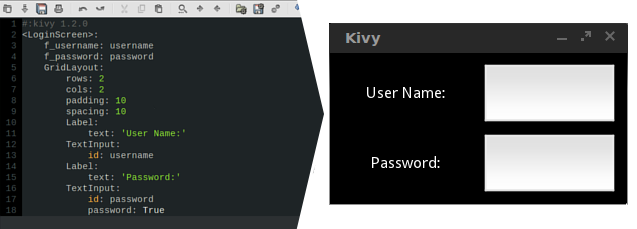
\includegraphics[width=0.99\textwidth]{kv-lang}
{\footnotesize\url{http://kivy.org/docs/gettingstarted/rules.html}}
\caption{KV Language para descripción de interfaces en Kivy}
\label{fig:kv-lang}
\end{figure}

Kivy~1.9 en aquel momento estaba en fase beta, y soportaba parcialmente Python~3. Sin embargo, sí funcionaba perfectamente para Python~2. No obstante, es de todos conocido los problemas de compatibilidad entre Python~3 y 2, y preferí usar el más reciente, Python~3, para el código del proyecto, por asegurar la aplicabilidad futura del proyecto. Hice algunas modificaciones en el núcleo de Kivy para modernizarlo,\footnote{Mis contribuciones al proyecto se pueden consultar en \url{https://github.com/kivy/kivy/pulls?q=is:pr+author:terrex+is:closed}} pero me estaba acumulando mucho retraso y lo abandoné en favor del lenguaje declarativo proporcionado por Qt conocido como QML.

\FloatBarrier
\newpage
\subsection{QML (Qt)}

Por contrapartida, las bibliotecas de Qt están bastante maduras. Se usan en el escritorio KDE desde siempre, y ha pasado a estar bajo el control de diferentes compañías ---Trolltech, Nokia, Digia---, que ofrecían diferentes licencias de uso, algo que siempre ha traído polémica en la comunidad de software libre alrededor de GNU/Linux.\footnote{\url{https://en.wikipedia.org/wiki/Qt_(software)\#Licensing}}
No obstante en los últimos años se han liberado versiones con licencias completamente compatibles con la definición de software libre de la \emph{Free Software Foundation}~(FSF).\index{FSF}

Qt también es multiplataforma, pero además ofrece una apariencia más integrada con el resto de la plataforma, ya que hace uso de las bibliotecas nativas para el renderizado de los elementos, sin tener un impacto visual reconocible dentro del ecosistema del sistema operativo (\autoref{fig:qt-multiplatform}).


\begin{figure}[htbp]
\centering
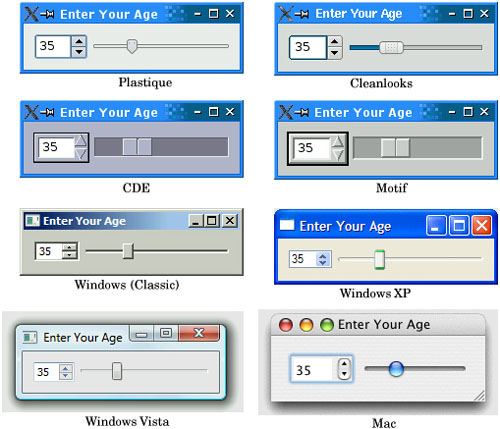
\includegraphics[width=0.7\textwidth]{qt-multiplatform}
{\footnotesize\url{http://www.veryhman.com/qt/ch01lev1sec3.html}}
\caption{Misma aplicación Qt en distintos entornos}
\label{fig:qt-multiplatform}
\end{figure}

A partir de la versión Qt~4.8, el framework incorpora el módulo QtQuick, que es el intérprete del lenguaje QML (acrónimo del inglés \emph{Qt Modeling Language})\index{QML}. Está basado en JavaScript, de manera que es muy similar al lenguaje KV de Kivy pero con más llaves \verb={}=, sólo que se permite toda la funcionalidad e interactividad que se pueda incorporar a través de JavaScript (ECMAScript). El documento base es una estructura en JSON (del inglés \emph{JavaScript Object Notation})\index{JSON} con la descripción de la interfaz en forma de árbol jerárquico.

Además, el framework ofrece su propio IDE llamado Qt~Creator, incluyendo un editor con reconocimiento de la sintaxis del lenguaje QML, algo que se agradece mucho.

Se puede ver un extracto del código QML en el \autoref{lst:qml-extract} que ha sido necesario para generar la pantalla de la \autoref{fig:qml-extract}. El problema principal con QML es la calidad de la documentación. Está desactualizada, y además se necesita mayor soporte de los elementos existentes en Qt para su uso desde QML.

\begin{figure}[htbp]
\centering
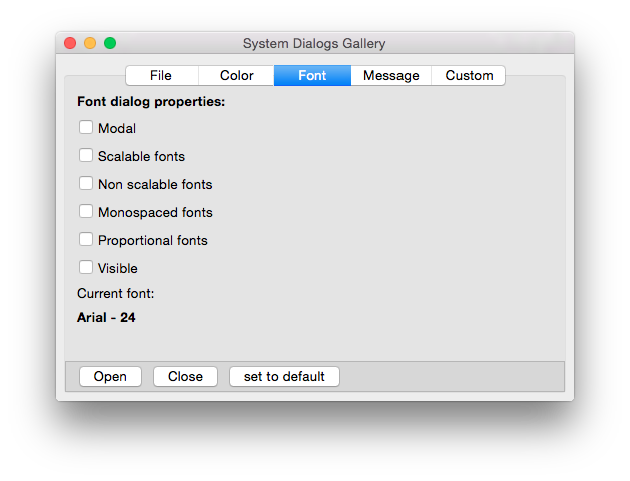
\includegraphics[width=0.8\textwidth,trim=56pt 80pt 56pt 30pt,clip]{qml-extract}
\caption{Aplicación de muestra de QtQuick (QML)}
\label{fig:qml-extract}
\end{figure}


\begin{listing}[phtb]
\begin{minted}[fontsize=\small]{js}
import QtQuick 2.2
import QtQuick.Controls 1.2

ApplicationWindow {
    title: "System Dialogs Gallery"
    width: 580
    height: 480

    TabView {
        /*...*/
        Tab {
            Column {
                id: optionsColumn
                anchors.fill: parent
                anchors.margins: 12
                spacing: 8
                Label {
                    font.bold: true
                    text: "Font dialog properties:"
                }
                CheckBox {
                    id: fontDialogModal
                    text: "Modal"
                    checked: true
                    Binding on checked { value: fontDialog.modality != Qt.NonModal }
                }
                CheckBox {
                    id: fontDialogScalableFonts
                    text: "Scalable fonts"
                    Binding on checked { value: fontDialog.scalableFonts }
                }
                /* ... */
                Label {
                    text: "Current font:"
                }
                Label {
                    id: fontLabel
                    text: "<b>" + fontDialog.font.family + " - " + fontDialog.font.pointSize + "</b>"
                    MouseArea {
                        anchors.fill: parent
                        onClicked: fontDialog.open()
                    }
                }
            }            
        }
        /*...*/
    }
}
\end{minted}
\caption{Extracto del QML de la aplicación de muestra}
\label{lst:qml-extract}
\end{listing}


El mayor problema que tuve fue la implementación de la tabla de datos. Según se extrae de la documentación, en QML existe el elemento \codep{TableView}, que debe incluir un \codep{TableViewColumn} para cada columna, clase que no tiene correspondencia en el Qt imperativo. Además, los datos deben ser provistos por filas, y una vez seleccionada la fila, tomar el dato de la columna necesaria; no permitiendo una matriz de filas y columnas de manera directa y accedido por la coordenada de la celda. Por eso es necesario reimplementar (\autoref{lst:MyTableModel}) un objeto con la interfaz \codep{QAbstractTableModel} y asignárselo vía Python en lugar de vía QML como cabría esperarse. No obstante una vez comprendido cómo se exportan los elementos de Qt a QML, se observa que es muy flexible, y que en el futuro, con un poco más de desarrollo, será QML completamente funcional y una alternativa real a la descripción imperativa de la interfaz.

\begin{listing}[htbp]
\begin{minted}{python}
from PyQt5.QtCore import QAbstractTableModel, QVariant, pyqtSlot, QModelIndex
import numpy as np

class MyTableModel(QAbstractTableModel):
    def __init__(self, headings, data):
        super().__init__()
        self.my_headings = headings
        if not hasattr(data, 'shape'):
            data = np.array(data)
        self.my_data = data

    @pyqtSlot(QModelIndex, result=int)
    @pyqtSlot(result=int)
    def rowCount(self, QModelIndex_parent=None, *args, **kwargs):
        return self.my_data.shape[0]

    @pyqtSlot(QModelIndex, result=int)
    @pyqtSlot(result=int)
    def columnCount(self, QModelIndex_parent=None, *args, **kwargs):
        return self.my_data.shape[1]

    @pyqtSlot(QModelIndex, int, result=QVariant)
    @pyqtSlot(QModelIndex, result=QVariant)
    def data(self, index: QModelIndex, role: int=None) -> QVariant:
        return str(self.my_data[index.row(), role - 32])

    @pyqtSlot(int, int, int, result=str)
    @pyqtSlot(int, int, result=str)
    def headerData(self, section: int, orientation: int, role: int=None):
        return self.my_headings[section]

    def roleNames(self):
        # los 32 primeros ``roles'' están reservados a Qt
        # para los roles personalizados, tenemos que empezar en el 32
        return dict(enumerate(self.my_headings, 32))
\end{minted}
\caption{Implementación de \codep{MyTableModel}}
\label{lst:MyTableModel}
\end{listing}

No obstante la complejidad del paquete QtQuick es bastante alta, y la potencia descriptiva de QML también. Tanto que la mayoría de los elementos de QML están implementados a su vez en el propio lenguaje QML, lo que denota una expresividad suficientemente versátil (\autoref{lst:qml-checkbox}).

\begin{listing}[phtb]
\begin{minted}[fontsize=\small]{js}
import QtQuick 2.2
import QtQuick.Controls 1.2
import QtQuick.Controls.Private 1.0
AbstractCheckable {
    id: checkBox
    property int checkedState: checked ? Qt.Checked : Qt.Unchecked
    property bool partiallyCheckedEnabled: false
    property bool __ignoreChecked: false
    property bool __ignoreCheckedState: false
    style: Qt.createComponent(Settings.style + "/CheckBoxStyle.qml", checkBox)
    activeFocusOnTab: true
    Accessible.role: Accessible.CheckBox
    Accessible.name: text
    __cycleStatesHandler: __cycleCheckBoxStates
    onCheckedChanged: {
        if (!__ignoreChecked) {
            __ignoreCheckedState = true;
            checkedState = checked ? Qt.Checked : Qt.Unchecked;
            __ignoreCheckedState = false;
        }
    }
    onCheckedStateChanged: {
        __ignoreChecked = true;
        if (checkedState === Qt.PartiallyChecked) {
            partiallyCheckedEnabled = true;
            checked = false;
        } else if (!__ignoreCheckedState) {
            checked = checkedState === Qt.Checked;
        }
        __ignoreChecked = false;
    }
    onPartiallyCheckedEnabledChanged: {
        if (exclusiveGroup && partiallyCheckedEnabled) {
            console.warn("Cannot have partially checked boxes in an ExclusiveGroup.");
        }
    }
    onExclusiveGroupChanged: {
        if (exclusiveGroup && partiallyCheckedEnabled) {
            console.warn("Cannot have partially checked boxes in an ExclusiveGroup.");
        }
    }
    function __cycleCheckBoxStates() {
        if (!partiallyCheckedEnabled) {
            checked = !checked;
        } else {
            switch (checkedState) {
                case Qt.Unchecked: checkedState = Qt.Checked; break;
                case Qt.Checked: checkedState = Qt.PartiallyChecked; break;
                case Qt.PartiallyChecked: checkedState = Qt.Unchecked; break;
}}}}
\end{minted}
\caption{\codet{CheckBox.qml}: Clase de QML \codep{CheckBox} implementada en el propio lenguaje QML}
\label{lst:qml-checkbox}
\end{listing}

\FloatBarrier
\section{Estructura y organización del código}

A continuación describimos la estructura y organización de directorios del proyecto.

\begin{itemize}
\item[] \blackdirectory{/memoria}\\
Ficheros fuentes \XeLaTeX, imágenes y scripts de recompilación de la memoria y presentación de diapositivas.
\item[] \blackdirectory{/project}\\
Ficheros fuentes raíz de Python. Incluye \path{logging.conf} y ficheros de ejemplo.
\item[] \blackdirectory{/project/pfcsamr}\\
Módulo principal.
\item[] \blackdirectory{/project/pfcsamr/gui.py}\\
Módulo \codep{pfcsamr.gui} con la implementación del Presentador del patrón MVP.
\item[] \blackdirectory{/project/pfcsamr/orchestrator.py}\\
Módulo \codep{pfcsamr.orchestrator} con la implementación del Modelo del patrón MVP.
\item[] \blackdirectory{/project/pfcsamr/Doc}\\
Documentación autogenerada del código usando el generador Sphinx.\footnote{\url{http://sphinx-doc.org}}
\end{itemize}

\FloatBarrier
\section{Acerca del rendimiento en Python}

Se observó que la carga del modelo entrenado \path{GoogleNews-vectors-negative300.bin.gz} consumía mucho tiempo y espacio ($\approx$\si{4.5}{GiB} y unos 5 minutos). Este modelo ha sido publicado por Google en el repositorio del proyecto \codep{word2vec} basado en el \emph{dataset} de Google News (aproximadamente 100 mil millones de palabras). El modelo contiene vectores 300-dimensionales para 3 millones de palabras y de frases (bigramas y trigramas). Las frases se obtuvieron usando una aproximación dirigida por datos sencilla, cuyo método se encuentra descrito en \cite{DBLP:journals/corr/MikolovSCCD13}.

Por ello se convirtió inicialmente el modelo del \emph{Word2Vec} original en la representación interna provista por \codep{gensim}, que soporta en \emph{unpickling} de datos de NumPy, de mejor desempeño.

El procedimiento para la conversión es:
\nopagebreak
\begin{listing}[H]
\begin{minted}{python}
from gensim.models.word2vec import Word2Vec
# lectura sin optimizar
model_orig = Word2Vec.load_word2vec_format('GoogleNews-vectors-negative300.bin', binary=True)
# escritura optimizada
model_orig.save('GoogleNews-vectors-negative300.bin.gensim')
\end{minted}
\caption{Conversión del formato crudo \codep{word2vec} en el optimizado por \codep{gensim}}
\label{lst:word2vec-convert}
\end{listing}

Y para la carga de la versión optimizada:
\nopagebreak
\begin{listing}[H]
\begin{minted}{python}
from gensim.models.word2vec import Word2Vec
# lectura optimizada
model = Word2Vec.load('GoogleNews-vectors-negative300.bin.gensim', mmap='r')
\end{minted}
\caption{Lectura del modelo optimizado por \codep{gensim} previamente almacenado}
\label{lst:word2vec-load}
\end{listing}
